\chapter{Remote Sensing Technologies and Platforms for Agricultural Monitoring}

\section{Introduction}
Remote sensing has become a key technology in modern agriculture, enabling efficient crop monitoring through aerial and satellite imagery. It allows for non-invasive observation of large agricultural areas, supporting early detection of stress and disease. 
This chapter introduces the main imaging technologies such as RGB, multispectral, and hyperspectral cameras. It also covers the platforms used for data collection, including satellites, aircraft, and UAVs. Vegetation indices and basic image processing techniques are explored to understand plant health. Lastly, practical applications of remote sensing in agriculture are highlighted.


\section{Imaging technologies in remote sensing}
Imaging technologies play a key role in remote sensing systems by capturing high-resolution images of the Earth’s surface, which are crucial for agricultural monitoring. These technologies use different types of cameras to detect various parts of the electromagnetic spectrum (Figure~\ref{fig:ImageAcquisition}), enabling detailed analysis of vegetation, soil, and environmental conditions. The choice of camera depends on the specific agricultural purpose, such as disease detection, crop monitoring, or environmental assessment.

\begin{figure}[H]
    \centering
    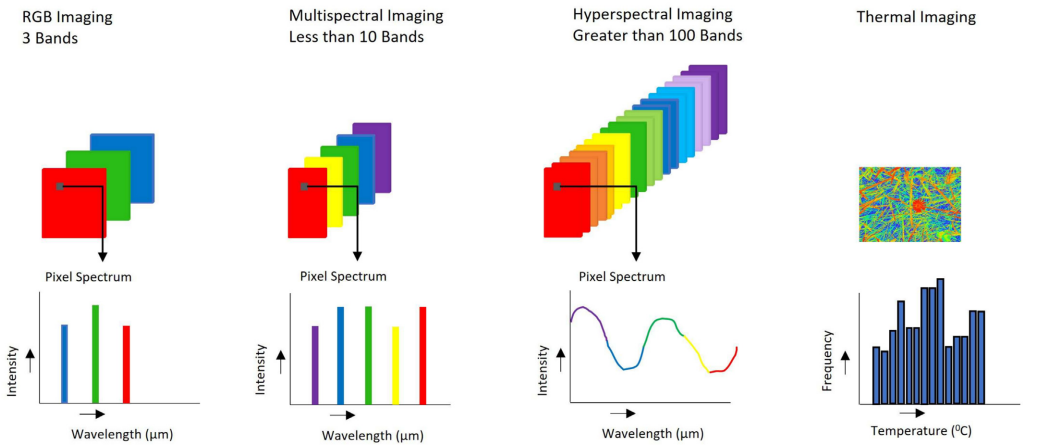
\includegraphics[width=\textwidth]{chapters/chapter01/images/Figure01.png}
    \caption{Image acquisition techniques \protect\parencite{ghazal2024computer}.}
    \label{fig:ImageAcquisition}
\end{figure}


\subsection{\gls{abb:rgb} cameras (Red, Green, Blue)}
\gls{abb:rgb} cameras are the most common type of imaging technology used in remote sensing. They capture images in the visible light spectrum (red, green, and blue wavelengths), similar to how the human eye perceives the world \parencite{delavarpour2021technical}.

\subsection{Near-Infrared (NIR) cameras}

Near-Infrared cameras capture images in the near-infrared spectrum, which lies just beyond the visible light range. These cameras are sensitive to light wavelengths that are not visible to the human eye, typically ranging from 700 to 1300 nm \parencite{delavarpour2021technical}. \gls{abb:nir} imaging is particularly valuable in plant health monitoring as it can detect subtle changes in vegetation that are not visible in the visible light spectrum.

\subsection{Thermal infrared cameras}

Thermal infrared cameras capture images based on the heat emitted by objects, operating in the infrared spectrum (wavelengths typically ranging from 8,000 to 14,000 nm). They detect temperature differences and translate them into visual representations, making them invaluable for identifying heat-related patterns in crops and soil \parencite{delavarpour2021technical}.


\subsection{Multispectral cameras}

Multispectral cameras capture images across multiple spectral bands, including visible (red, green, blue) and non-visible wavelengths (near-infrared and red-edge) across a limited number of discrete bands, each covering a wider spectral range spanning tens to hundreds of nanometers \parencite{lu2020recent}. These cameras typically have 5 to 10 bands, enabling detailed analysis of plant health and environmental conditions \parencite{delavarpour2021technical}. They are essential for applications that require data beyond what RGB cameras can provide.

\subsection{\gls{abb:lidar} cameras (Light Detection and Ranging)}

\gls{abb:lidar} cameras use laser pulses to measure distances by calculating the time it takes for the laser to bounce back from a surface. This technology generates high-resolution 3D maps, capturing detailed information about the shape and structure of the terrain, vegetation, and other objects. \gls{abb:lidar} operates effectively in various environmental conditions, including low light or dense canopy cover \parencite{delavarpour2021technical}.

\subsection{Hyperspectral cameras}
Hyperspectral cameras capture images across a vast range of continuous, narrow spectral bands, often exceeding hundreds. These bands typically have a spectral resolution below 10 nanometers, covering both visible and non-visible wavelengths. The fine-scale spectral data collected allows for the detection of subtle variations in reflectance, enabling detailed analysis of crop conditions, such as disease identification and nutrient stress. This high-resolution imaging is crucial for precision agriculture, where detecting subtle differences can significantly impact decision-making and yield optimization \parencite{delavarpour2021technical} \parencite{lu2020recent}.

\section{Remote Sensing platforms}
Remote sensing platforms are categorized based on their altitude and mobility, each offering unique capabilities for capturing agricultural data. The three main types are satellite-based imaging, UAV (drone) imaging, and aircraft imaging.

\subsection{Satellite-Based imaging}
Satellite-based imaging involves the use of Earth-observing satellites equipped with multispectral sensors to capture detailed images of the Earth's surface. These satellites, such as Quickbird and Landsat-1, can capture high-resolution images, providing data with varying levels of precision. Early satellite systems offered up to 6.5 meters per pixel in resolution \parencite{phang2023satellite}, while modern systems have significantly improved both spatial and spectral resolution. These advancements enable more accurate and comprehensive monitoring of large areas, laying the foundation for a wide range of applications, including agriculture and environmental studies \parencite{adao2017hyperspectral}. Despite its many advantages, satellite-based imaging also presents several challenges and limitations that must be considered in agricultural applications, including:

\begin{itemize}
    \item \textbf{Coarse Resolution:} The resolution of satellite imagery can be too coarse for some applications. For instance, imagery from platforms like Sentinel-2 (up to 10 m resolution) may not be detailed enough for fields with closely spaced rows, such as vines, leading to mixed pixel data that combines multiple rows and soil \parencite{adao2017hyperspectral}.
    
    \item \textbf{Data Processing Complexity:} Due to the coarse resolution, advanced methods like computer vision classifiers and statistical decision trees are often required to extract useful information, such as detecting shrubs or distinguishing plant species \parencite{phang2023from}.
    
    \item \textbf{Mixed Pixel Issue:} Low-resolution pixels, like those from Landsat, result in mixed data, complicating analysis and interpretation, especially in detailed applications \parencite{delavarpour2021technical}.
    
    \item \textbf{Spatiotemporal Challenges:} Obtaining timely spatiotemporal data on crop phenological status during critical growth periods is difficult, especially due to cloud coverage \parencite{delavarpour2021technical}.
    
    \item \textbf{High Costs:} Accessing satellite data equipped with multispectral sensors can be expensive, which limits its use for some applications \parencite{delavarpour2021technical}.
  \end{itemize}
  

\subsection{Aircraft-Based imaging}

Aircraft-based imaging involves the use of piloted or unpiloted aircraft, such as airplanes, equipped with various remote sensing tools to capture high-resolution imagery and sensor data over large agricultural areas. These systems offer a significant advantage in large-scale applications due to their flexibility and ability to carry heavier payloads of sensors, making them a viable alternative to satellite-based or \gls{abb:uav}-based solutions \parencite{delavarpour2021technical}.
Before the widespread adoption of \gls{abb:uav}s, manned aircraft were commonly employed for lower-to-ground remote sensing, utilizing multi-spectral or electro-optic (EO) sensors to monitor agricultural conditions \parencite{phang2023satellite}, However, this approach also faces several limitations, including:

\begin{itemize}
    \item \textbf{High Operational Costs:} Operating aircraft-based systems involves significant expenses for fuel, maintenance, and pilot salaries, making them less affordable compared to UAVs \parencite{delavarpour2021technical, phang2023from}.
    
    \item \textbf{Complex Logistics and Pilot Requirement:} Certified pilots and specific flight logistics are essential, adding complexity and reducing flexibility in deployment \parencite{adao2017hyperspectral}.
    
    \item \textbf{Limited Flexibility:} Aircraft require designated takeoff and landing zones, restricting their use in remote or uneven terrains \parencite{delavarpour2021technical}.
    
    \item \textbf{Weather Sensitivity:} Adverse weather conditions, such as strong winds or rain, can impact flight stability and data quality, limiting operations during critical periods \parencite{delavarpour2021technical}.
    
    \item \textbf{Regulatory and Airspace Restrictions:} Aircraft-based systems are subject to strict aviation regulations and airspace restrictions, limiting their operational scope \parencite{delavarpour2021technical}.
    
    \item \textbf{High Data Processing Requirements:} Large volumes of data generated require specialized software and computing resources, making data processing resource-intensive \parencite{delavarpour2021technical}.
    
    \item \textbf{Costly for Large-Scale Use:} The expense and complexity of these systems make them impractical for frequent large-scale monitoring, favoring UAV alternatives for cost efficiency \parencite{phang2023from}.
    
    \item \textbf{Resolution Limitations:} Although aircraft provide better resolution than satellites, their imagery can still be too coarse for some precision applications \parencite{adao2017hyperspectral}.
  \end{itemize}
  
\subsection{\gls{abb:uav}-Based imaging}

Unmanned Aerial Vehicles (\gls{abb:uav}s), or drones, are versatile remote sensing platforms that have become essential tools in remote sensing due to their cost-effectiveness, flexibility, and ability to capture high-resolution (cm-level) images, making them ideal for precision agriculture \parencite{sishodia2020applications}. \gls{abb:uav}-based imaging typically involves using low-altitude remote Sensing Systems to acquire detailed imagery of the Earth’s surface at low altitudes, providing high precision and adaptability \parencite{phang2023satellite}.

Unlike traditional satellite platforms, \gls{abb:uav}s offer several advantages, including on-demand data collection, high-resolution imagery, and flexible deployment, which enable real-time monitoring and analysis \parencite{phang2023satellite}. A complete Unmanned Aerial System (UAS) includes the \gls{abb:uav} and its remote sensing equipment, operating without a human pilot onboard, and is capable of carrying various sensors tailored to different agricultural needs \parencite{adao2017hyperspectral}, Despite their advantages, \gls{abb:uav}s also face some challenges, including:

\begin{itemize}
    \item \textbf{Short Flight Duration:} \gls{abb:uav}s, especially smaller models, often have flight durations of less than 30 minutes, which limits their coverage area, particularly for large-scale agricultural operations \parencite{phang2023from}.
    
    \item \textbf{Regulatory Challenges:} Stricter regulations, especially for larger \gls{abb:uav}ss, slow down their adoption and innovation, hindering their widespread use \parencite{phang2023from, delavarpour2021technical}.
    
    \item \textbf{Scalability:} \gls{abb:uav}-based remote sensing requires trained pilots and continuous monitoring, which limits scalability, particularly for small-scale applications \parencite{phang2023from}.
    
    \item \textbf{Environmental Sensitivity and Calibration Issues:} Hyperspectral sensors on \gls{abb:uav}ss face challenges related to environmental factors such as light exposure and atmospheric interference, necessitating frequent recalibration \parencite{adao2017hyperspectral}.
    
    \item \textbf{Weather Dependency:} \gls{abb:uav}s are susceptible to weather conditions like wind and rain, which can affect both flight stability and data quality \parencite{delavarpour2021technical}.
    
    \item \textbf{Battery Life:} The limited battery life of \gls{abb:uav}ss impacts their ability to cover large areas, particularly in extensive agricultural fields \parencite{delavarpour2021technical}.
  \end{itemize}
  
\section{Vegetation indices}
Vegetation indices are mathematical formulas that combine light reflectance data from different spectral bands (such as visible, near-infrared, and mid-infrared) captured by sensors on drones or satellites to assess plant health and condition. These indices provide valuable insights into growth stages, plant vigor, biomass, and chlorophyll levels \parencite{sishodia2020applications}. Plants reflect sunlight differently based on their type, structure, and water content: they reflect little in the blue and red regions, more in green (which makes them appear green), and strongly in the near-infrared (\gls{abb:nir}) if healthy (Figure~\ref{fig:bluegreenred}). 

\begin{figure}[H]
    \centering
    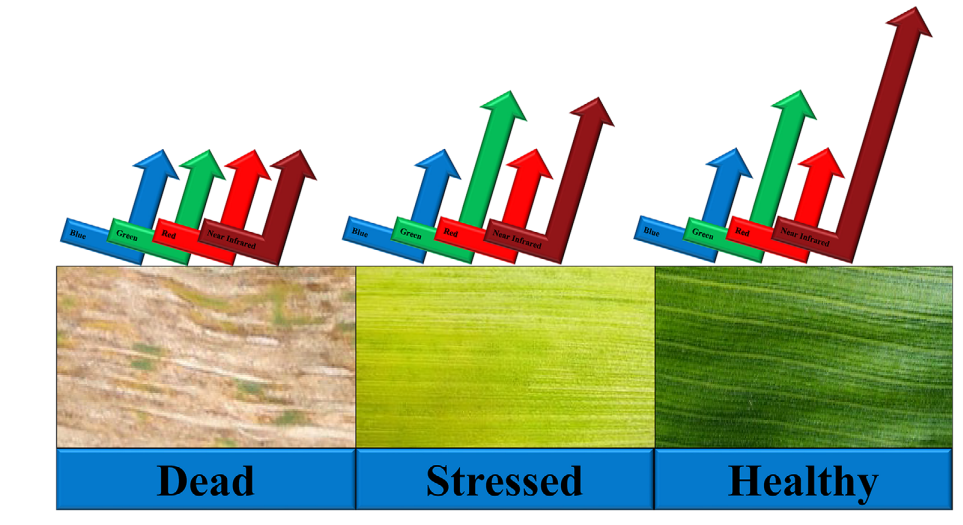
\includegraphics[width=0.8
    \textwidth]{chapters/chapter01/images/Figure05.png}
    \caption{Unique optical reflectance signature differences of blue, green, red, and near-infrared light emitted from dead, stressed, and healthy plant tissue \protect\parencite{olson2021review}.}
    \label{fig:bluegreenred}
\end{figure}


Thermal and infrared indices, including CWSI (Crop Water Stress Index) and SIWSI (Shortwave Infrared Water Stress Index), use thermal radiation data to estimate plant temperature, water stress, and transpiration, aiding in drought detection, crop yield estimation, and disease monitoring \parencite{sishodia2020applications}. For more vegetation indices, their mathematical formulas, and detailed applications, refer to Appendix~\ref{app:annexA}.
\begin{table}[htbp]
    \caption{
        Some recently used vegetation indices for remote sensing applications in precision agriculture \parencite{sishodia2020applications}. \\
        \textbf{Note:} \textit{Red, Green, and Blue} refer to visible bands of the electromagnetic spectrum. \textit{NIR (Near-Infrared)} refers to wavelengths (~700–1300 nm). \textit{Red Edge} is the narrow spectral region (~680–750 nm) between the red and NIR bands.
    }
    \centering
    \resizebox{\textwidth}{!}{%
    \begin{tabular}{|p{4cm}|p{5cm}|p{6cm}|}
    \hline
    \textbf{Spectral Index} & \textbf{Equation} & \textbf{Application} \\
    \hline
    Normalized Difference Vegetation Index (NDVI) & $NDVI = \frac{\text{NIR} - \text{Red}}{\text{NIR} + \text{Red}}$ & Measure of healthy, green vegetation \\
    \hline
    Green Normalized Difference Vegetation Index (GNDVI) & $GNDVI = \frac{\text{NIR} - \text{Green}}{\text{NIR} + \text{Green}}$ & Measure of healthy, green vegetation; higher chlorophyll concentration sensitivity than NDVI \\
    \hline
    Red Edge Normalized Difference Vegetation Index (RENDVI) & $RENDVI = \frac{\text{NIR} - \text{Red Edge}}{\text{NIR} + \text{Red Edge}}$ & Modification of NDVI; utilizes the red edge for enhanced sensitivity to vegetation stress \\
    \hline
    Soil Adjusted Vegetation Index (SAVI) & $SAVI = \frac{1.5(\text{NIR} - \text{Red})}{\text{NIR} + \text{Red} + 0.5}$ & Modification of NDVI; suppresses the effects of soil pixels \\
    \hline
    Atmospherically Resistant Vegetation Index (ARVI) & $ARVI = \frac{\text{NIR} - (\text{Red} - \text{Blue})}{\text{NIR} + (\text{Red} - \text{Blue})}$ & Designed to be less affected by atmospheric conditions; used for disease and weed mapping \\
    \hline
    Wide Dynamic Range Vegetation Index (WDRVI) & $WDRVI = \frac{\text{NIR} - \text{Red}}{\text{NIR} + \text{Red}}$ & N-Application, yield estimation, crop growth (LAI), and disease detection \\
    \hline
    Normalized Difference Red Edge Index (NDRE) & $NDRE = \frac{\text{NIR} - \text{Red Edge}}{\text{NIR} + \text{Red Edge}}$ & Used for crop yield estimation, biomass, nitrogen management, and disease detection \\
    \hline
    Red Edge Difference Vegetation Index (REDVI) & $REDVI = \text{NIR} - \text{Red Edge}$ & Estimates biomass, nitrogen uptake, and nutrient concentration \\
    \hline
    \end{tabular}%
    }
    \label{tab:vegetation-indices}
\end{table}





\section{Image processing}

Imagery processing is the technique used to turn multiple aerial images captured by drones (\gls{abb:uav}s) or remote sensors into a single, accurate, and clear image known as an orthomosaic. Since drones don’t capture one large image but instead take many smaller ones of different parts of the area, these images must be merged using a process called image stitching  (as shown in Figure~\ref{fig:UAVDataProducts}), This involves merging individual images into one large composite by identifying and aligning “key points” such as a rock, plant, or edge of a field. While the drone captures these images, it simultaneously records \gls{abb:gps} or location metadata, which is then used in geographic alignment to position each image on a map accurately. The final output of this process is known as data products, which can include color mosaics (stitched colored images), spectral mosaics (capturing invisible wavelengths like near-infrared for agricultural analysis), thermal mosaics (highlighting temperature variations), surface and terrain models (representing elevation and landscape shapes), and point clouds (dense 3D representations of surfaces for detailed analysis) \parencite{olson2021review}.

\begin{figure}[H]
    \centering
    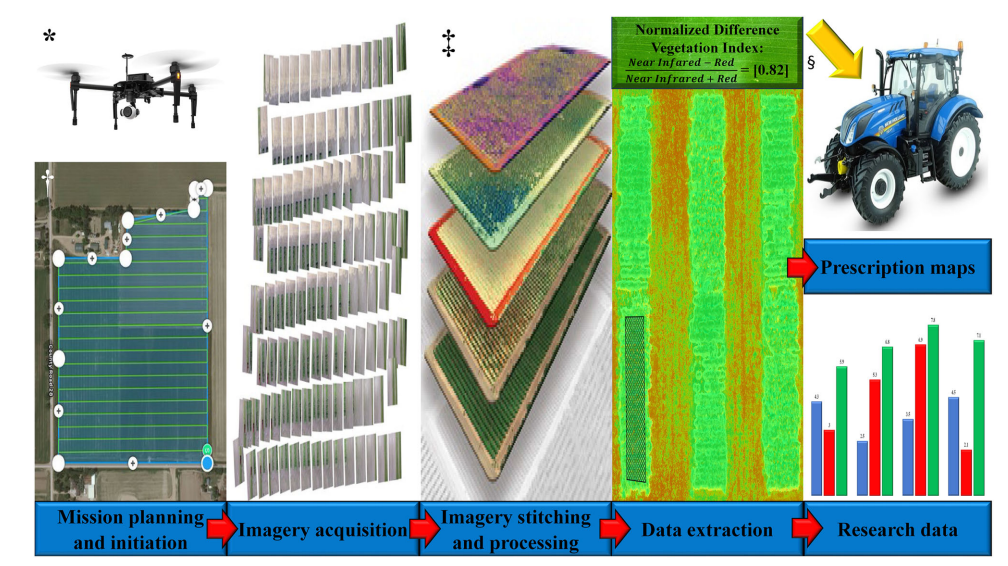
\includegraphics[width=0.9
    \textwidth]{chapters/chapter01/images/Figure06.png}
    \caption{Standard Workflow for Generating \gls{abb:uav}-Derived Imagery and Data Products \protect\parencite{olson2021review}.}
    \label{fig:UAVDataProducts}
\end{figure}

Imagery can be processed on-site with personal computers and the appropriate software or in the field with cloud computing imagery processing \parencite{olson2021review}. The pros and cons of each imagery processing option are discussed in Table~\ref{tab:ProcessingMethodComparison}.

\begin{table}[h]
    \centering
    \renewcommand{\arraystretch}{1.5} % Increase row height
    \setlength{\tabcolsep}{8pt} % Adjust column padding
    \begin{tabular}{|p{3cm}|p{5.5cm}|p{5.5cm}|}
    \hline
     & \textbf{Pros} & \textbf{Cons} \\ \hline
    
     \multirow{4}{*}{\parbox{2.8cm}{\centering\textbf{Software (On-Site Processing on PC)}}}    & Customizable options & High-performance PC needed \\ \cline{2-3}
    & No limits on images & Expensive initial cost \\ \cline{2-3}
    & GIS software compatible & Steep learning curve \\ \cline{2-3}
    & One-time purchase & Slower processing \\ \hline
    
    \multirow{4}{*}{\parbox{2.8cm}{\centering\textbf{Cloud Computing (Online/Remote Processing)}}}    & Easy to use & Fewer customizations \\ \cline{2-3}
    & Low upfront cost & Image limits \\ \cline{2-3}
    & Fast field processing & Ongoing costs \\ \cline{2-3}
    & No powerful PC needed & \\ \cline{2-3}
    & Simplified analysis & \\ \hline
    \end{tabular}
    \caption{Comparison of On-Site Software vs. Cloud Computing for Imagery Processing \parencite{olson2021review}.}
    \label{tab:ProcessingMethodComparison}
    \end{table}
    

\section{Applications of remote sensing data}
Remote sensing has diverse applications in agriculture, enabling precise, data-driven decision-making. It helps monitor field conditions, optimize resource use, and address issues early. The following sections highlight key areas where remote sensing enhances farm management:

\begin{itemize}[leftmargin=1.5em]

    \item \textbf{Crop Health Monitoring:} Remote sensing enables regular monitoring of crop conditions, helping detect diseases, pest presence, and water or nutrient stress early. Vegetation indices (e.g., NDVI) derived from \gls{abb:rgb}, \gls{abb:nir}, multi-spectral, and hyperspectral sensors are commonly used to assess aspects such as foliage cover, pigment composition, and water stress. \gls{abb:lidar} and \gls{abb:gps} can also support the accurate mapping of plant structure and spatial positioning. These technologies collectively support better crop management and yield optimization \parencite{phang2023satellite}.
    
    \item \textbf{Weed Control:} Precise weed detection helps reduce competition for water, nutrients, and light. Aerial imagery from \gls{abb:uav}s and satellite platforms, often using \gls{abb:rgb} and multispectral cameras, supports vegetation indexing and mapping for weed identification. Some systems enable real-time onboard image analysis and spraying. These tools assist in implementing targeted and efficient weed management strategies while reducing input costs \parencite{phang2023satellite}.
    
    \item \textbf{Infectious Disease Epidemiology and Mapping:} \gls{abb:uav}s are used to gather high-resolution spatial data for studying the relationships between environmental conditions and disease spread. They help monitor changes in land use, population distribution, and vegetation patterns, which are valuable for identifying and mitigating disease risks affecting crops or livestock. UAV-collected data provide flexible, cost-effective alternatives to satellite and manned aerial surveys \parencite{phang2023satellite}.
    
    % \item \textbf{Spectral Imaging:} Multispectral and hyperspectral imaging technologies offer detailed insights into crop nutrient levels, stress, and overall vigor. Though hyperspectral data offer higher spectral resolution, they also require more complex processing, often conducted post-flight. These systems rely on sensors like CCD and CMOS and use scanning methods such as point, line, and plane scanning. Accurate georeferencing is achieved using ground control points (GCPs) or advanced navigation systems \parencite{phang2023satellite}.
    
\end{itemize}


\section{Conclusion}
In this chapter, we explored the foundations of remote sensing technologies and their crucial role in agricultural monitoring, particularly for detecting plant stress and diseases. We reviewed various imaging systems, data acquisition platforms, and key vegetation indices used to assess crop health. While remote sensing provides rich and valuable data, its full potential is unlocked when combined with intelligent analysis methods. In the next chapter, we shift focus to another technological domain, deep learning and computer vision, which offer powerful tools for automating and enhancing the interpretation of agricultural imagery, especially for disease recognition in wheat crops